\documentclass[11pt,english,french]{scrreprt}
\usepackage{lmodern}
\usepackage{babel}
\renewcommand{\familydefault}{\rmdefault}
\usepackage[T1]{fontenc}
\usepackage{ucs}
\usepackage[utf8x]{inputenc}
\usepackage[a4paper]{geometry}
\geometry{verbose,tmargin=2cm,bmargin=2cm,lmargin=2cm,rmargin=2cm,headheight=2cm,footskip=1cm}
\setlength{\parskip}{\smallskipamount}
\setlength{\parindent}{0pt}

\usepackage{amsthm}
\usepackage{booktabs}
\usepackage{amsmath}
\usepackage[unicode=true, pdfusetitle,
 bookmarks=true,bookmarksnumbered=false,bookmarksopen=false,
 breaklinks=false,pdfborder={0 0 1},backref=false,colorlinks=false]
 {hyperref}

\makeatletter
\usepackage{colortbl}
\usepackage{color}
\usepackage[dvipsnames]{xcolor}
\usepackage{wrapfig}
\usepackage{graphicx}
\usepackage{listings}
\usepackage[calcwidth]{titlesec}
\usepackage{fix-cm}
\usepackage{multicol}
\usepackage{verbatim}
\usepackage{moreverb}
\usepackage{nicefrac}
\usepackage{amssymb}
\usepackage{array}
\usepackage{tabularx}
\usepackage{subfig}
\usepackage[french,ruled,vlined]{algorithm2e}
\SetAlgoProcName{Procédure}{proc}

\theoremstyle{remark}
  \newtheorem*{rem*}{Remarque}
\theoremstyle{definition}
  \newtheorem*{defi}{Définition}
  \newtheorem{ques}{Question}[section]
  \newtheorem{idee}{Idée}[ques]

\definecolor{MyDarkBlue}{rgb}{0,0.08,0.45}

\lstset{language=C,
	 	basicstyle=\small\ttfamily,
		keywordstyle=\small\ttfamily,
		identifierstyle=,
		commentstyle=\textcolor{OliveGreen},
		columns=fullflexible,
		stringstyle=\small\ttfamily,
		showstringspaces=false,numberstyle=\tiny, breaklines=false, tabsize=4}

\titleformat{\section}[hang]{\sffamily\bfseries}
 {\Large\thesection}{12pt}{\Large}[{\titlerule[0.5pt]}]

\def\thickhrulefill{\leavevmode \leaders \hrule height 1pt\hfill \kern \z@}
\renewcommand{\maketitle}{\begingroup%
    \let\footnotesize\small
    \let\footnoterule\relax
    \parindent \z@
    \reset@font
    \begin{flushleft}
      \huge \sffamily \bfseries\color{orange} \@title
    \end{flushleft}
    \hrule height 1pt
    \begin{flushright}
      \large\sffamily\color{MyDarkBlue}\@author
    \end{flushright}
  \endgroup%
  \setcounter{footnote}{0}%
}

\AtBeginDocument{
  \def\labelitemi{\normalfont\bfseries{--}}
}

\makeatletter
\renewcommand\thesection{\arabic{section}}
\@addtoreset{section}{chapter}
\makeatother

\makeatother
\begin{document}
	
\title{LI310 - Examen 2008 -- Rattrapage\\
Mercredi 14 janvier 2009}
\author{Benjamin BARON}

\maketitle

\section{Couche physique} % (fold)

A l'aide d'une connexion WiFi, un point d'accès transmet à un utilisateur A de la vidéo ayant les caractéristiques suivantes : une image est constituée d'une matrice $1024\times 768$ pixels, chaque pixel pouvant prendre une valeur parmi 64 possibles. La vidéo est transmise à raison de 23 images par seconde.

\begin{ques}
	Le débit de transmission du point d'accès est exprimé par la formule :\[D=\log_2(64)\times 1024\times 768\times 23 = 108,53\;\textrm{Mbit/s}\]
	
	Il faut donc un débit de transmission égal à 108,53 Mbit/s.
\end{ques}

\begin{ques}
	Avec la technologie WiFi, la largeur de bande est de 10 MHz, située entre $5\,000$ MHz et $5,\,010$ MHz, et les interférences imposent un rapport signal-à-bruit $\nicefrac{S}{N}$ égal à 31 dB.
	
	D'après la loi de Shannon, la capacité du canal de transmission est exprimée par :\[C=B\log_2\left(1+\frac{P_S}{P_N}\right)\]
	Or \[\frac{P_S}{P_N}=10^{\frac{\nicefrac{S}{N}}{10}}=1258,93\]
	
	Ainsi, on a :\[C=B\log_2\left(1+\frac{P_S}{P_N}\right)=10.10^6\times\log_2(1+1258,93)=102,99\;\textrm{Mbit/s}\]
	
	De ce fait, on ne peut pas transmettre ce signal sur ce canal car $C < D$.
\end{ques}

Grâce à de nouvelles technologies sans fil, il est possible de cumuler les débits sur plusieurs bandes de fréquences. En effet, dans notre cas nous allons pouvoir transmettre une partie du débit sur la bande WiFi $[5\,000,\,5\,010]$ MHz, et le reste sera placé sur un autre canal.

\begin{ques}
	On considère que le canal WiFi peut transporter un débit maximal de $D'=68,5$ Mbit/s. De plus, le codage possède une valence de $M=64$ (codé sur $r=6$ bits).
	
	La largeur de la bande la bande passante du canal complémentaire doit satisfaire la loi de Nyquist : \[D\leqslant 2B\log_2(M)\Leftrightarrow B \geqslant \frac{D-D'}{2\log_2(M)} = \frac{(108,53-68,5).10^6}{2\times\log_2(64)}=3,33\;\textrm{MHz}\]
	
	Ainsi, la bande passante du canal complémentaire doit avoir une valeur minimale de 3,33 MHz.
\end{ques}

En réalité, un canal de bande passante $[5\,010,\,5\,014]$ MHz est disponible, cependant ce canal subi des interférences qui rendent son rapport signal-à-bruit égal à 20 dB.

\begin{ques}
	D'après la loi de Shannon, la capacité $C$ de ce canal est alors exprimée par :\[C=B\log_2\left(1+\frac{P_S}{P_N}\right)=B\log_2\left(1+10^{\frac{\nicefrac{S}{N}}{10}}\right)= 4.10^6\times \log_2\left(1+10^{\frac{20}{10}}\right)=26,63\;\textrm{Mbit/s}\]
\end{ques}

\begin{ques}
	Les bandes de fréquences choisies sont proches l'une de l'autre : $[5\,000,\,5\,010]$ et $[5\,010,\,5\,014]$. Il risque donc d'y avoir des interférences, ce qui provoquera une dégradation des performances.
	
	Les paramètres qui affectent les performances du canal sans-fil sont :\begin{itemize}
		\item Les interférences ;
		\item La présence d'un autre équipement évoluant dans la même bande de fréquences ($\Rightarrow$ collisions) ;
		\item La présence d'un autre réseau sans-fil ;
		\item La distance entre la source du réseau sans-fil et le récepteur.
	\end{itemize}
\end{ques}

\begin{ques}
	Un réseau sans-fil est seulement \emph{half-duplex} -- HDX (ie. le système fournit ne communication dans les deux sens, mais seulement une seule direction à la fois).
	
	De ce fait, les calculs effectués ne restent pas valables si A envoie également de la vidéo vers le point d'accès.
\end{ques}

\section{LAN} % (fold)

On souhaite construire un réseau local avec $N$ machines utilisateurs dont la topologie logique est un \textbf{anneau} et la topologie physique est une \textbf{étoile}. Les machines sont toutes à une distance $L$ de la machine centrale, la vitesse de propagation d'un signal est $V$ et le débit de toutes les machines est $D$. Les trames sont de tailles $T$ avec un entête de taille $E$ (inclus dans $T$). La traversée de la machine centrale est toujours instantanée (simple récepteur). La taille du jeton est négligeable.

Pour les applications numériques, on prendra : $N=100,\;D=5$ Mbit/s, $L=100$ m, $V=2.10^8$ m/s, $T=1\,000$ bits, $E=50$ bits.

\begin{ques}
	Représentation graphique de la topologie physique en indiquant le chemin suivi par un paquet sur cette topologie.
	\begin{figure}[h]
		\center
		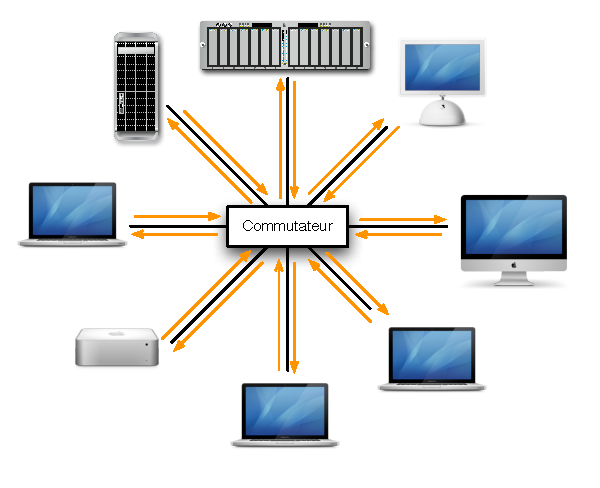
\includegraphics[scale=.8]{Exam2009/etoile-phy}
	\end{figure}
\end{ques}

\begin{ques}
	Temps de transmission $t_{trans}$ et de propagation $t_{prop}$ d'une machine à la suivant sur l'anneau.
	\[t_{trans} = \frac{T}{D}=\frac{1\,000}{5.10^6}=200\;\mu\textrm{s}\]
	\[t_{prop} = \frac{2L}{V} = \frac{2\times 100}{2.10^8}=1\;\mu\textrm{s}\]
\end{ques}

\begin{ques}
	Dans chacun des cas suivants, calculer le temps total séparant la réception du jeton (par une machine ayant une trame à transmettre sur l'anneau) de sa libération (par la même machine). En déduire l'efficacité de chaque technique.
	
	L'efficacité $e_i$ d'une technique se mesure par la formule :\[e_i = \frac{t_{transmission}}{t_{occupation\_support}}\]
	\begin{idee}
		On suppose que toutes les machines utilisateurs doivent avoir reçu une trame complète avant de pouvoir la retransmettre. La station émettrice doit attendre le retour complet de sa propre trame pour réinjecter le jeton sur l'anneau.
		
		On a alors : 
		\begin{eqnarray*}
		T_{1} & = & N\times\left(t_{prop}+t_{trans}\right)\\
		T_{1} & = & 100\times\left(1.10^{-6}+200.10^{-6}\right)=20,1\;\textrm{ms}
		\end{eqnarray*}
		\[e_1 = \frac{t_{trans}}{T_1} = \frac{0,2}{20,1} = 0,00995\approx 1\%\]
	\end{idee}
	
	\begin{idee}\label{ques:3.b}
		Dès réception de l'en-tête complet une machine peut commencer à retransmettre la trame ou libérer le jeton.
		
		On suppose que la station émettrice doit attendre le retour complet de sa propre trame pour libérer le jeton.\\
		On a alors :
		\begin{eqnarray*}
		T_{2} & = & N\times\left(t_{prop}+\frac{E}{D}\right)\\
		T_{2} & = & 100\times\left(1.10^{-6}+\frac{50}{5.10^{6}}\right)=1,1\;\textrm{ms}
		\end{eqnarray*}
		\[e_2 = \frac{t_{trans}}{T_2} = \frac{0,2}{1,1} = 0,1818 \approx 18,18\%\]
	\end{idee}
	
	\begin{idee}\label{ques:3.c}
		La machine destinataire doit lire toute la trame avant de la retransmettre vers l'émetteur mais toutes les autres peuvent retransmettre la trame ou libérer le jeton dès réception de l'en-tête.
		
		De même, on suppose que la station émettrice doit attendre le retour complet de sa propre trame pour libérer le jeton.\\
		On a alors :
		\begin{eqnarray*}
		T_{3} & = & (N-1)\times\left(t_{prop}+\frac{E}{D}\right)+t_{trans}+t_{prop}\\
		T_{3} & = & (100-1)\times\left(1.10^{-6}+\frac{50}{5.10^{6}}\right)+200.10^{-6}+1.10^{-6}=1,29\;\textrm{ms}
		\end{eqnarray*}
		\[e_3 = \frac{t_{trans}}{T_3} = \frac{0,2}{1,29} = 0,155\approx 15,5\%\]
	\end{idee}
\end{ques}

\begin{ques}
	On considère le scénario suivant : à $T_0$, les machines 1, 2 et 100 veulent transmettre une trame et la machine 1 possède le jeton.
	
	Description de tous les évènements significatifs pour les machines 1, 2 et 100 jusqu'à la libération du jeton par 100. On considère le fonctionnement de la question \ref{ques:3.c}.
	
	\begin{tabularx}{\textwidth}{llX}
		\toprule 
		Instant & Jeton & Evénement\tabularnewline
		\midrule
		\midrule
		$T_0$ & 1 & 1, 2 et 100 veulent transmettre ; 1 transmet\tabularnewline
		\midrule 
		$T_{99}$ & 1 & 1 reçoit sa trame et libère le jeton\tabularnewline
		\midrule 
		$T_{100}$ & 2 & 2 reçoit le jeton et transmet sa trame\tabularnewline
		\midrule 
		$T_{199}$ & 2 & 2 reçoit sa trame et libère le jeton\tabularnewline
		\midrule 
		$T_{296}$ & 100 & 100 reçoit le jeton et envoie sa trame\tabularnewline
		\midrule 
		$T_{295}$ & 100 & 100 reçoit sa trame et libère le jeton\tabularnewline
		\bottomrule
	\end{tabularx}
\end{ques}

\begin{ques}
	On souhaite avoir une efficacité maximale. Il faut alors choisir le fonctionnement \ref{ques:3.c} -- 3.b. De plus, il faut modifier les paramètres :\begin{itemize}
		\item Diminution de $L$;
		\item Augmentation de $D$;
		\item Diminution de $T$.
	\end{itemize}
\end{ques}

\section{Commutation et routage} % (fold)

Soit un réseau d'entreprise composé de plusieurs réseaux locaux reliés par des ponts. La topologie du système est donnée par la figure suivante :
\begin{figure}[h]
	\center
	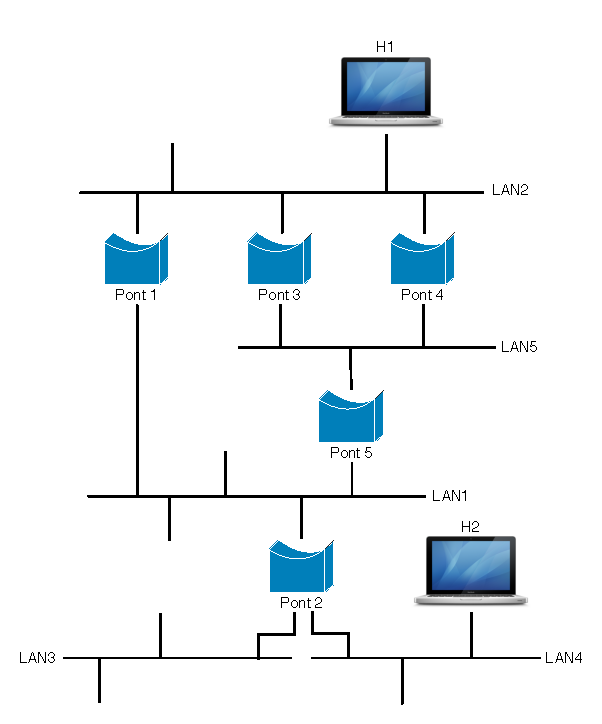
\includegraphics[scale=1]{Exam2009/LAN}
\end{figure}

\begin{ques}
	Un réseau ainsi constitué peut fonctionner car il existe au moins un chemin reliant deux stations entre elles.
\end{ques}

\begin{ques}
	Le protocole \emph{Spanning Tree Protocol} (STP) --- IEEE 802.1D est utilisé dans les ponts afin d'éviter les boucles qui apparaissent lorsque la topologie est un graphe connexe. Ce protocole permet de remplacer une topologie de graphe connexe par un arbre couvrant permettant de sélectionner un chemin unique entre chaque station du réseau (le résultat est donc un arbre reliant tous les ponts à partir d'un pont \emph{racine}).
	
	Représentation possible du réseau logique utilisé dans ce cas si le pont 1 est la racine :
	\begin{figure}[h]
		\center
		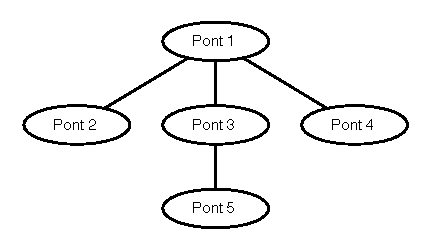
\includegraphics[scale=1]{Exam2009/STP}
	\end{figure}
\end{ques}

\begin{ques}
	Un autre protocole appelé \emph{Source Routing Bridging} (SRB) --- IEEE 802.2 est maintenant utilisé à la place du SPT. Les LANs sont de type Ethernet. Ce protocole revient à identifier tous les chemins de la source vers une destination.
	
	Il faut pouvoir repérer le chemin choisi par la source. Il faut donc ajouter un champ identifiant le chemin emprunté dans la trame Ethernet (\emph{routing information field} --- RIF).
\end{ques}

\begin{ques}
	Les chemins possibles en SR de H1 vers H2 sont :\begin{itemize}
		\item $C_1\colon$ H1 $\rightarrow$ Pont 4 $\rightarrow$ Pont 5 $\rightarrow$ Pont 2 $\rightarrow$ H2
		\item $C_2\colon$ H1 $\rightarrow$ Pont 3 $\rightarrow$ Pont 5 $\rightarrow$ Pont 2 $\rightarrow$ H2
		\item $C_3\colon$ H1 $\rightarrow$ Pont 1 $\rightarrow$ P2 $\rightarrow$ H2
	\end{itemize}
	
	Le chemin $C_3$ est le plus court. Si l'on considère la même pondération sur toutes les liaisons du réseau, il serait alors choisi par la source H1.
\end{ques}

\begin{ques}
	Avantages / désavantage des deux protocoles.
	
	\begin{tabularx}{\textwidth}{lXX}
		\toprule 
		& \emph{Spanning Tree Protocol} & \emph{Source Routing}\tabularnewline
		\midrule
		\midrule
		Avantages & Simple à mettre en place ; préservation de la transparence (aucune modification nécessaire de la trame) & La source peut choisir un chemin optimal ; robuste et systématique\tabularnewline
		\midrule
		Inconvénients & Nécessité de surveiller les liaisons (messages de contrôle + estampillage des trames) ; n'utilise pas tous les liens pour étaler la charge ; Les ponts redondants ne sont pas utilisés; un seul chemin entre deux ponts du réseau &  Phase d'apprentissage coûteuse (diffusion totale) ; difficile à gérer pour de grands réseaux\tabularnewline
		\bottomrule
	\end{tabularx}
\end{ques}

\clearpage

\section{IP} % (fold)

On dispose de deux réseaux A et B reliés entre eux par une passerelle (\emph{getway}). Le réseau A est également relié à Internet par une passerelle.

Réseau A : \lstinline!metaux-net! adresse IP : 192.3.2.0 \begin{itemize}
	\item Masque de sous-réseau : 255.255.255.0
	\item Ordinateur 1 : \lstinline!platine! adresse IP 192.3.2.2 interface eth0
	\item Ordinateur 2 : \lstinline!uranium! adresse IP 192.3.2.3 interface eth0
	\item Serveur \lstinline!mercure! adresse IP 192.3.2.4 interface eth0
\end{itemize}

Réseau B : \lstinline!roches-net! adresse IP 130.2.0.0 \begin{itemize}
	\item Masque de sous-réseau : 255.255.254.0
	\item Ordinateur 1 : \lstinline!quartz! adresse IP 130.2.0.2 interface eth0
	\item Ordinateur 2 : \lstinline!silex! adresse IP 130.2.0.3 interface eth0
\end{itemize}

La passerelle entre le réseau A et le réseau B a deux interfaces :\begin{itemize}
	\item eth0 : \lstinline!pass-versA! adresse IP 192.3.2.1
	\item eth1 : \lstinline!pass-versB! adresse IP 130.2.0.1
\end{itemize}

Les noms des différentes machines seront utilisés à la place des adresses MAC (Ethernet).

\begin{figure}[h]
	\center
	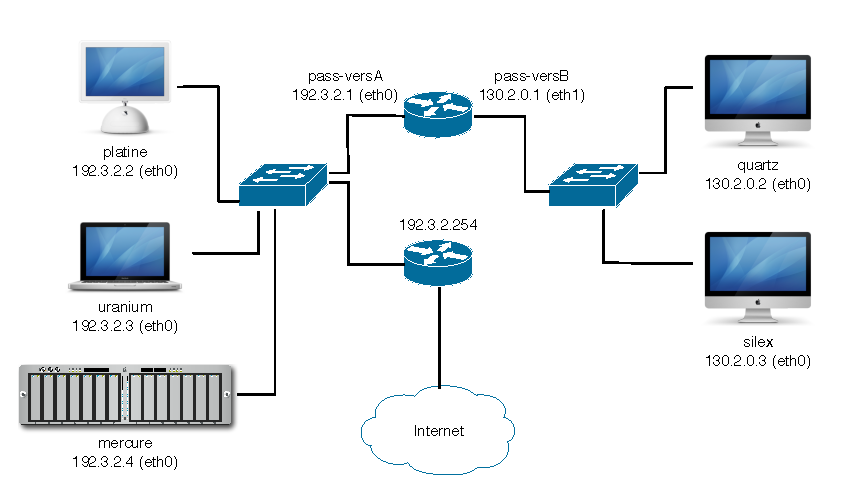
\includegraphics[scale=.8]{Exam2009/Reseau}
\end{figure}

\begin{ques}
	Le réseau A a pour adresse IP 192.3.2.0. Or $192_d = 1100\,0000_b$. Donc c'est une adresse de classe C et le masque primaire est 255.255.255.0, ce qui est le masque utilisé. Le réseau A n'a donc pas été subdivisé.
	
	Le réseau B a pour adresse IP 130.2.0.0. Or $130_d = 1000\,0010_b$. Donc c'est une adresse de classe B et le masque primaire est 255.255.0.0, qui est différent du masque utilisé. Le réseau B a donc été subdivisé.
\end{ques}

\begin{ques}
	Le réseau A comporte déjà 5 terminaux (2 ordinateurs, 1 serveur et 2 passerelles) et son masque de sous-réseau est 255.255.255.0. On peut alors ajouter $2^8-(5+2) = 249$ machines supplémentaires.
	
	Le réseau B comporte 3 terminaux (2 ordinateurs et une passerelle) et son masque de sous-réseau est 255.255.254.0. On peut alors ajouter $2^9-(3+2) = 507$ machines supplémentaires.
\end{ques}

\begin{ques}
	Adresse de diffusion :\begin{itemize}
		\item Réseau A : 192.3.2.255/24
		\item Réseau B : 130.2.1.255/23
	\end{itemize}
\end{ques}

\begin{ques}
	Table de routage minimale d'une machine du réseau A : 
	
	\begin{tabularx}{\textwidth}{XXXX}
		\toprule 
		Destination & Masque & Passerelle & Interface\tabularnewline
		\midrule
		\midrule
		default & 0.0.0.0 & 192.3.2.254 & eth0\tabularnewline
		\midrule
		130.2.0.0 & 255.255.254.0 & 192.3.2.1 & eth0\tabularnewline
		\bottomrule
	\end{tabularx}
	
	Table de routage minimale d'une machine du réseau B :
	
	\begin{tabularx}{\textwidth}{XXXX}
		\toprule 
		Destination & Masque & Passerelle & Interface\tabularnewline
		\midrule
		\midrule
		default & 0.0.0.0 & 130.2.0.1 & eth0\tabularnewline
		\midrule
		192.3.2.0 & 255.255.255.0 & 130.2.0.1 & eth0\tabularnewline
		\bottomrule
	\end{tabularx}
	
	Table de routage minimale de la passerelle entre le réseau A et le réseau B :
	
	\begin{tabularx}{\textwidth}{XXXX}
		\toprule 
		Destination & Masque & Passerelle & Interface\tabularnewline
		\midrule
		\midrule
		default & 0.0.0.0 & 192.3.2.254 & eth0\tabularnewline
		\midrule
		192.3.2.0 & 255.255.255.0 & {*} & eth0\tabularnewline
		\midrule
		130.2.0.0 & 255.255.254.0 & {*} & eth1\tabularnewline
		\bottomrule
	\end{tabularx}
\end{ques}

\begin{ques}
	La machine \lstinline!quartz! (130.2.0.2) souhaite ouvrir une connexion http avec le serveur \lstinline!mercure! (192.3.2.4). Donner les champs manquants des quatre trames transportant le segment SYN et le segment SYN/ACK.
	
	Trame transportant le segment SYN
	\begin{figure}[h]
		\center
		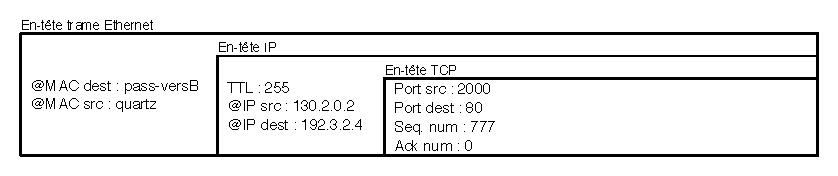
\includegraphics[scale=.8]{Exam2009/SYN-quartz}
		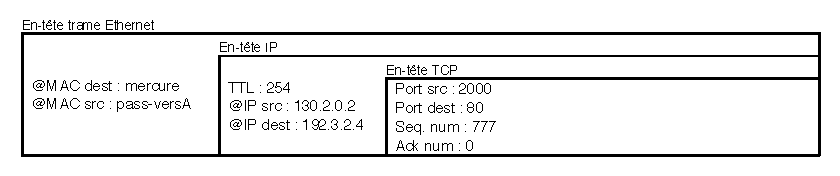
\includegraphics[scale=.8]{Exam2009/SYN-pass}
	\end{figure}
	
	Trame transportant le segment SYN/ACK
	\begin{figure}[h]
		\center
		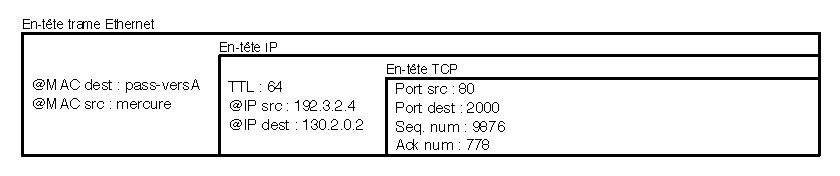
\includegraphics[scale=.8]{Exam2009/SYNACK-mercure}
		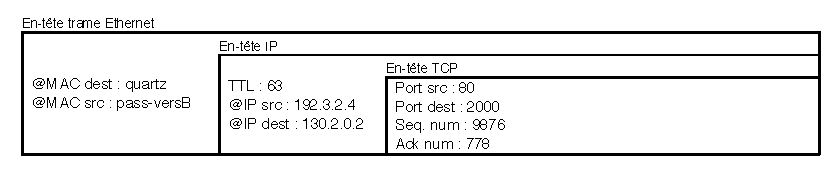
\includegraphics[scale=.8]{Exam2009/SYNACK-pass}
	\end{figure}
\end{ques}
\end{document}